\subsection{2D NMR: HSQC}
\label{subsec:theory__hsqc}

The use of coherence orders is particularly effective in the analysis of modern 2D NMR experiments, which make use of multiple different techniques to select for particular \textit{coherence transfer pathways} (CTPs).
A full discussion of this is beyond the scope of this thesis.
Nevertheless, the analysis of a 2D \proton{}--\carbon{} HSQC experiment (\cref{fig:hsqc_1grad}) is given here as an example to illustrate the concepts of CTP selection through \textit{phase cycling} and gradients, as well as the related issue of quadrature detection in indirect dimensions.

\begin{figure}[ht]
    \centering
    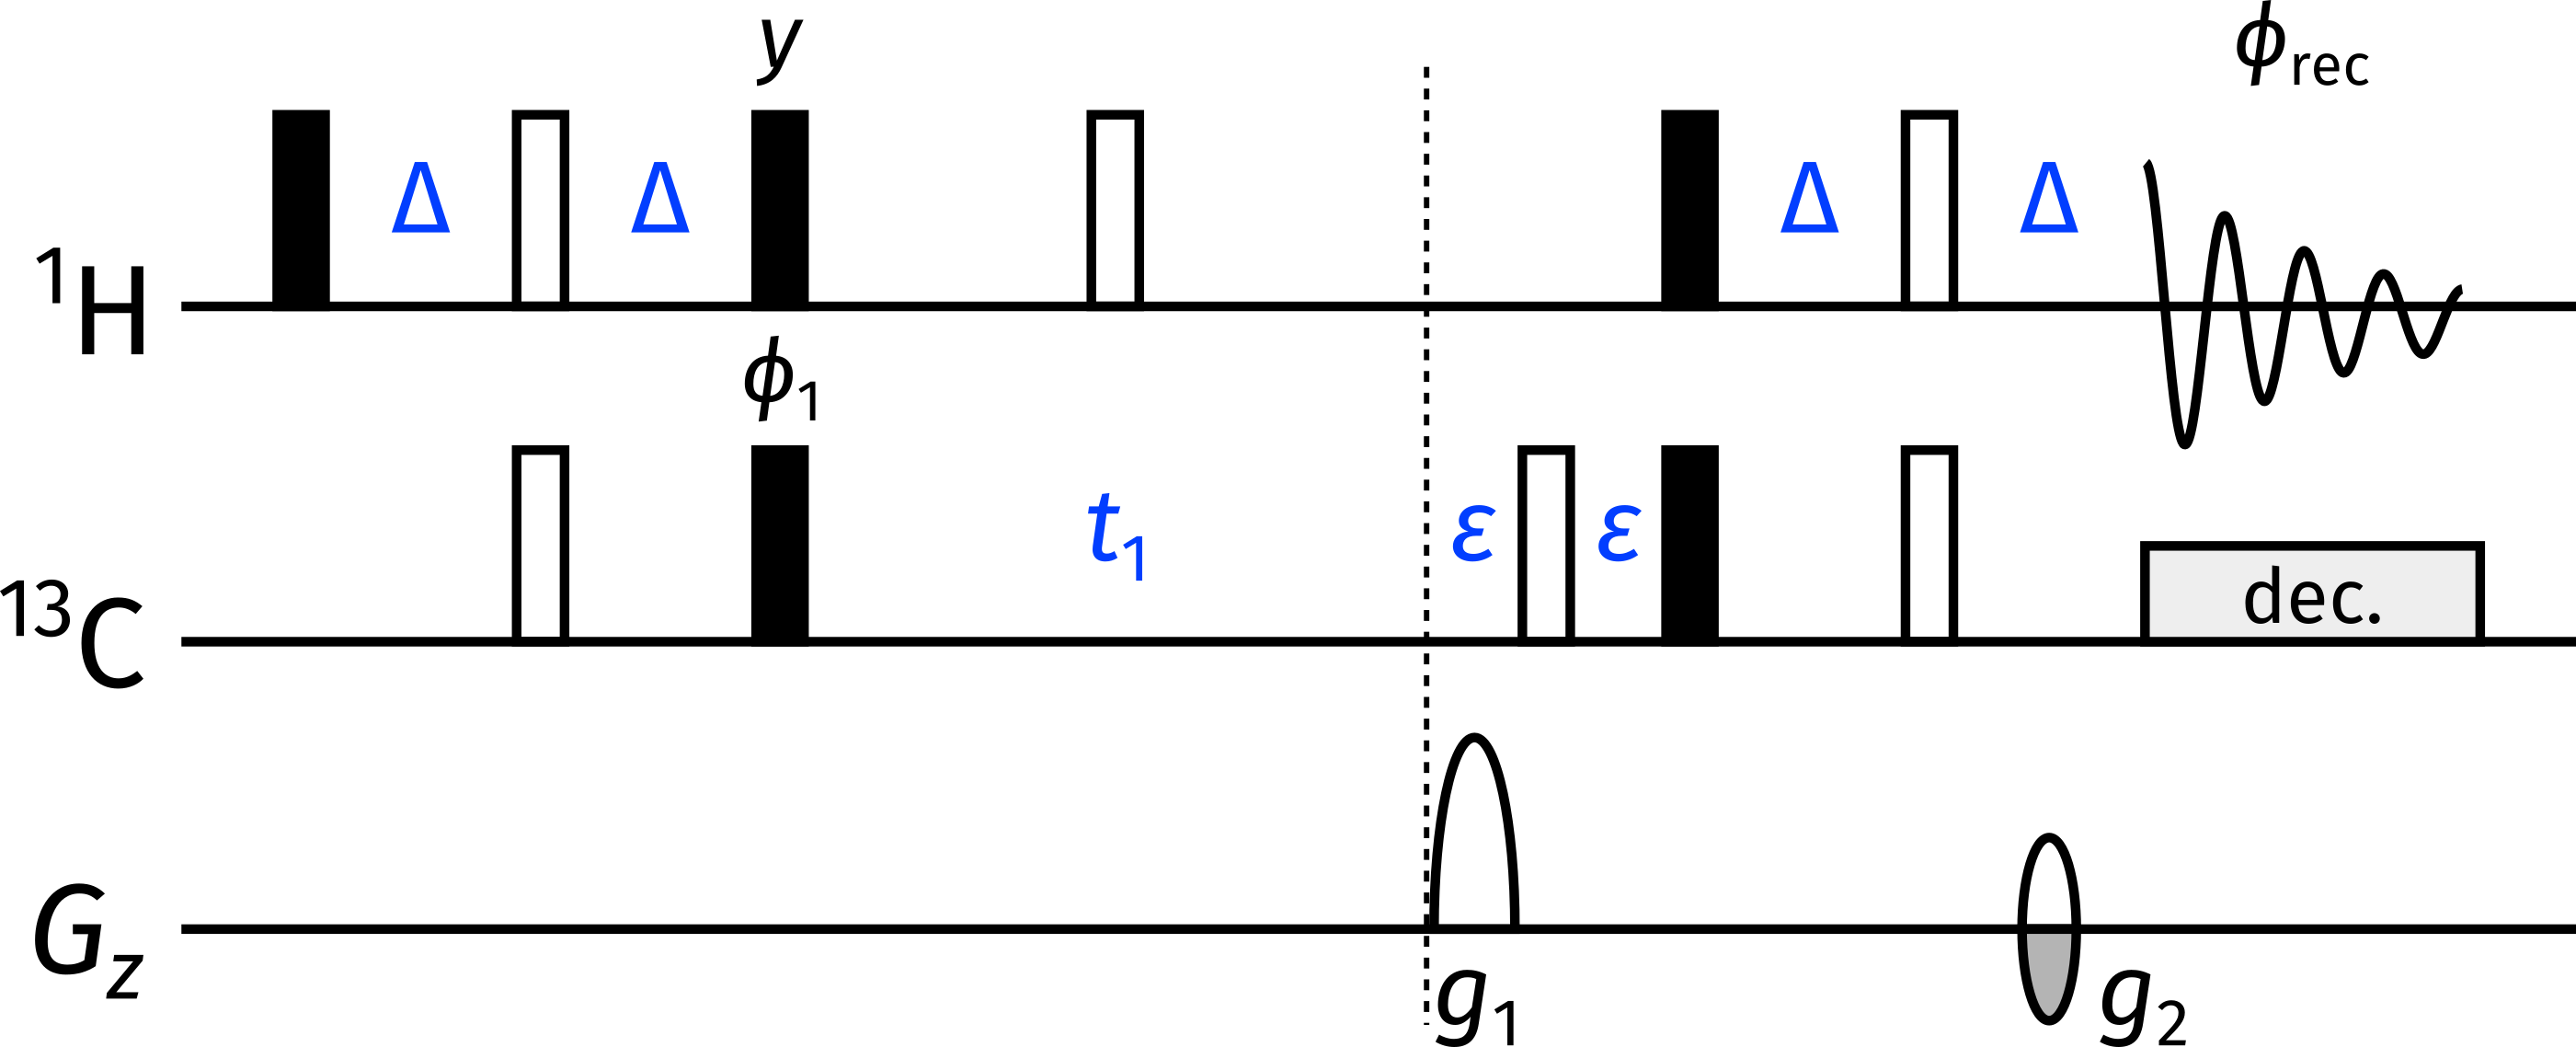
\includegraphics[scale=1.2]{pp/hsqc/hsqc_1grad.png}
    \caption[Echo--antiecho HSQC pulse sequence]{
        A typical echo--antiecho HSQC pulse sequence (the symbols are explained in the \textit{Preface}).
        The pulse phase $\phi_1$ and the receiver phase $\phi_\text{rec}$ are together alternated between $0$ and $\pi$; this is typically denoted as $\phi_1 = \phi_\text{rec} = (x, -x)$ as these phases correspond to the $+x$- and $-x$-axes.
        The delay $\Delta$ is set to $1/(4 \cdot \oneJ{CH})$.
        The gradient amplitudes are chosen such that $|g_1/g_2| = \gamma_{\ch{H}}/\gamma_{\ch{C}} \approx 4$.
        Echo--antiecho CTP selection is carried out by inverting the sign of $g_2$.
    }
    \label{fig:hsqc_1grad}
\end{figure}

The HSQC experiment seeks to only detect protons directly bonded to \carbon{}; all other protons must be suppressed.
We first show how pulsed field gradients and phase cycling allow the \textit{desired} signal to be obtained.

\todo{
This is technically only appropriate for an isolated methine (i.e. \ch{CH}) group.
The analysis which proceeds, however, is identical for methylene and methyl groups, which would be $I_2S$ and $I_3S$ systems respectively.
More unsound is the complete neglect of \ch{H}--\ch{H} coupling.
Luckily, this does not pose a serious problem here: it essentially leads to a small loss of signal.
However, for other experiments it may be necessary to account for $\nJ{HH}$: for example, it causes artefacts in the sensitivity-enhanced HSQC, as will be discussed in \cref{subsec:noah__sehsqc}.
In general, this illustrates the point that one should choose the \textit{simplest possible system} (but not one any simpler) to analyse a pulse sequence.
}


\todo{
\begin{itemize}
    \item CTP selection through gradients, mathematical requirement for CTP to be refocused
    \item Quadrature detection in $F_1$ (ugh)
    \item Composite coherence order\autocite{John1991JMR,Mitschang1995JCP}
    \item phase cycling to cancellation of unwanted peaks (e.g.\ arising from \ch{^{12}C}-bound \ch{^{1}H})
    \item explain why phase cycling (on its own) isn't really used for CTP selection any more
\end{itemize}
}
